% !TeX root = presentation.tex
% !TeX spellcheck = de_DE

\documentclass[presentation.tex]{subfiles}

\begin{document}
	
    \begin{frame}{Chaostheorie}{Szenario 1}
    	\begin{columns}
    		\begin{column}{.5\textwidth}
    			\begin{table}
    				\begin{tabular}{ | c | c |}
    					\hline
						 $ \rho $ & 22 \\\hline
						 $ \sigma $ & 10 \\\hline
						 $ \beta $ & 2.666 \\\hline
    				\end{tabular}
    			\end{table}
    		\end{column}
    		\begin{column}{.5\textwidth}
    			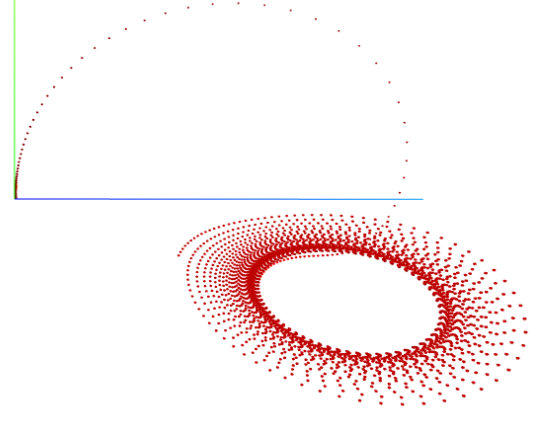
\includegraphics[width=\textwidth]{Chaostheorie1}
    		\end{column}
    	\end{columns}
	    \only<handout>{Da wir in der Klimatologie die Anomalien studieren, möchten wir euch zwei Anomalien im Lorenz-Model zeigen. Die erste betrifft die sprunghafte Änderung der Form und der Ausgabe des Models bei kleiner Änderung der Parameter.}
    \end{frame}
    \begin{frame}{Chaostheorie}{Szenario 2}
    	\begin{columns}[T]
    		\begin{column}{.5\textwidth}
    			\begin{table}
    				\begin{tabular}{ | c | c |}
    					\hline
    					$ \rho $ & 24.7 \\\hline
    					$ \sigma $ & 10 \\\hline
    					$ \beta $ & 2.666 \\\hline
    				\end{tabular}
    			\end{table}
    		\end{column}
    		\begin{column}{.5\textwidth}
    			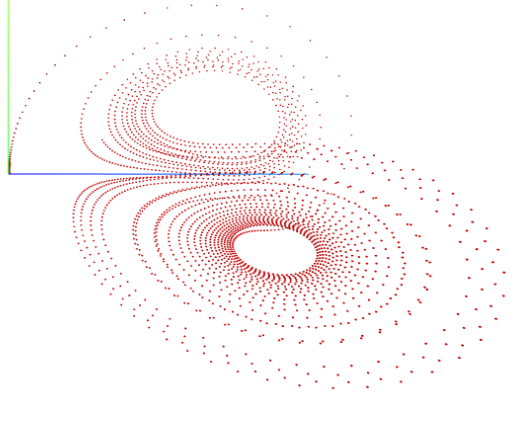
\includegraphics[width=\textwidth]{Chaostheorie2}
    		\end{column}
    	\end{columns}
	    \only<handout>{Auch wenn rho danach auf 24.69 gesetzt wird(delta -0.01) verändert sich die Form um den letzten Punkt erheblich. Der letzte Punkt befindet sich ganz an einem anderen Ort -> chaotisches Verhalten (minimste Parameteränderungen führen zu grossen Änderungen der Werte)
	    	Dennoch bleibt Grundform des Modells aber erhalten}
    \end{frame}
\end{document}